\subsection{Evolutionäre Algorithmen}
\flqq Unter evolutionären Algorithmen (EA) verstehen wir randomisierte Heuristiken, die Suchprobleme näherungsweise durch vereinfachende algorithmische Umsetzung von Prinzipien der natürlichen Evolution zu lösen versuchen. Somit geben evolutionäre Algorithmen in der Regel weder eine Garantie bezüglich der benötigten Rechenzeit noch der Güte der ausgegebenen Lösung. Ein Suchproblem besteht darin, zu einer Zielfunktion ein Element aus deren Definitionsbereich zu finden, dessen Funktionswert möglichst gut ist. Darunter verstehen wir im Folgenden, wenn nicht ausdrücklich anders vermerkt, einen möglichst grossen Funktionswert, weshalb der Zielfunktionswert eines Elements auch als seine Fitness bezeichnet wird.

Der Aufbau eines evolutionären Algorithmus lässt sich dann grob wie folgt beschreiben: in jedem Schritt verwaltet er eine Menge fester Grösse von Suchpunkten, die so genannte \Gls{population}, wobei jeder einzelne Suchpunkt auch als \Gls{individuum} bezeichnet wird. Aus den Punkten der Population neue Punkte zu erzeugen, ist Aufgabe von Mutation und Rekombination. Dabei steht hinter der Mutation die Idee, jeweils nur ein einzelnes Individuum zufällig zu verändern, ohne dass andere Individuen dabei berücksichtigt werden. Durch Rekombination wird hingegen aus mehreren, meist zwei Individuen zufällig ein neues gebildet, das von diesen möglichst gute Eigenschaften übernehmen soll. Durch Mutation und Rekombination werden also neue Individuen (Kinder genannt) aus bestehenden Individuen (Eltern genannt) erzeugt. Beide Operatoren hängen oftmals stark von Zufallsentscheidungen ab. Jedoch fliesst in der Regel weder in Mutation noch Rekombination der Zielfunktionswert der Individuen ein.

Die Zielfunktion beeinflusst nur die Selektion. Dieser Operator wählt Individuen der Population aus, sei es zur Auswahl der Eltern für eine Rekombination oder Mutation oder, um aus der Menge von Eltern und Kindern die nächste Population zu wählen, was den Übergang zur nächsten Generation darstellt. Dadurch, dass die Selektion Punkte mit höherem Zielfunktionswert mit grösserer Wahrscheinlichkeit auswählt, soll erreicht werden, dass nach und nach immer bessere Punkte gefunden werden.\frqq \cite{droste}

\begin{figure}[h]
  \centering
  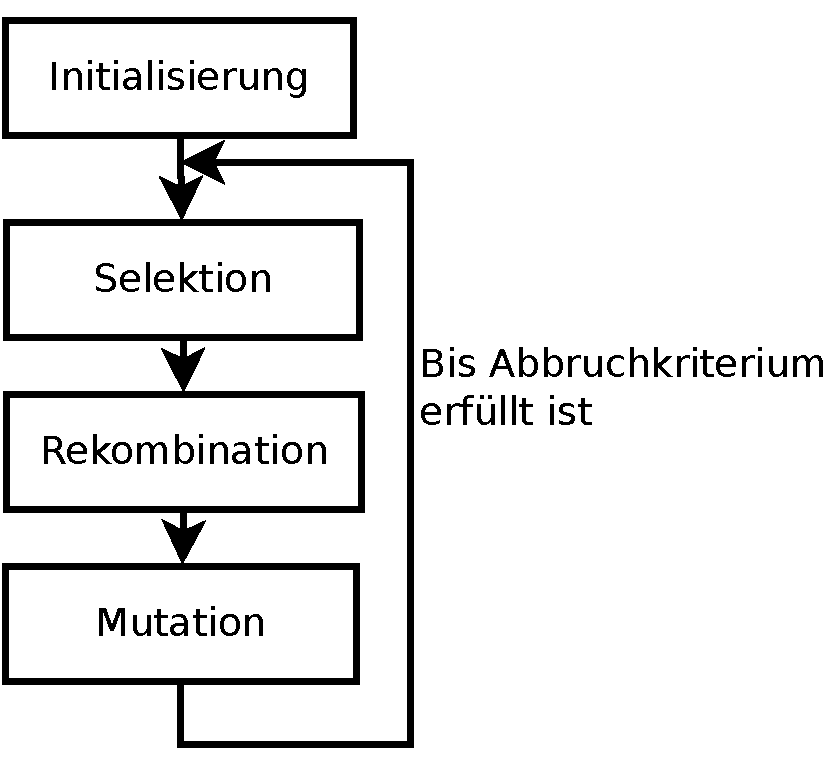
\includegraphics[width=0.5\textwidth]{images/evolutionaerer_algorithmus.pdf}
  \caption[Evolutionärer Algorithmus]{Evolutionärer Algorithmus \cite{droste}}
  \label{fig:evolutionary_algorithm}
\end{figure}

\subsubsection{Anwendung auf unser Problem}
Unser Problem der Findung von regulären Automaten welche die selbe Sprache akzeptieren wie ein gegebener regulärer Ausdruck, lässt sich mit einigen Anpassungen in diesem Standardmodell eines evolutionären Algorithmus abbilden.

\paragraph{Initialisierung}
In der Initialisierungsphase wird eine Population von Automaten zufällig erzeugt. Das heisst eine eine zufällige Anzahl von Zuständen wird erzeugt, diese werden Zufällig miteinander verbunden und zum Schluss wird ein zufälliger Startzustand und eine Menge von akzeptierenden Zuständen festgelegt.

\paragraph{Selektion}
Es werden jeweils diejenigen Automaten selektiert welche eine höhere Fitness aufweisen.

\paragraph{Problemmenge}
Die Problemmenge ist eine Menge von Tupeln ($Wort$, $Soll Ausgabe$) welche verwendet wird um die Fitness von Automaten zu bestimmen. Im Rahmen dieser Arbeit werden verschiedene Ansätze zur Erzeugung und zum Verhalten solcher Problemmengen ausprobiert. Dabei wird das Konvergenzverhalten des evolutionären Algorithmus untersucht.

\paragraph{Fitness}
Die Fitness von Automaten wird durch ausprobieren verschiedener Problemen und dem darauf folgenden Vergleich der Ausgabe mit einer Soll-Ausgabe bestimmt. Die Soll Ausgabe wird mithilfe des gegebenen regulären Ausdrucks bestimmen. Der Wert der Fitnessfunktion entspricht der Anzahl richtig gelöster Probleme aus der entsprechenden Problemmenge.

\textbf{Definitionen:}\\
$P$ = Problemmenge (Menge von Tupeln)\\
$P_i$ = i-tes Element aus der Problemmenge (Tupel ($Wort$, $Soll Ausgabe$))\\
$P_{i1}$ = 1. Element (Wort) des i-ten Elementes aus der Problemmenge\\
$P_{i2}$ = 2. Element (Soll Ausgabe; $1$ oder $0$) des i-ten Elementes aus der Problemmenge\\
$p$ = Anzahl Elemente in der Problemmenge $P$\\

\begin{equation}
Automat(Wort) = \left\{ 
 \begin{array}{l l}
   1 & \quad \text{Wenn das Wort akzeptiert wird}\\
   0 & \quad \text{Wenn nicht}
 \end{array} \right.\\
\end{equation}

\begin{equation}
equal(x, y) = \left\{ 
 \begin{array}{l l}
   1 & \quad \text{Wenn x und y gleich sind}\\
   0 & \quad \text{Wenn nicht}
 \end{array} \right.
\end{equation}

\begin{equation}
fitness(Automat, P) = \sum_{i=1}^{p} equal(Automat(P_{i1}), P_{i2})\\
\end{equation}

Daraus folgt:\\
\begin{equation}
   \begin{split}
	\max fitness(Automat, P) = p\\
	\min fitness(Automat, P) = 0
   \end{split}
\end{equation}

\paragraph{Rekombination}
Wenn man zwei endliche Automaten graphisch zusammenfügt, wird der resultierende Automat ein komplett anderes Verhalten aufweisen als die beiden Eltern. Deshalb verzichten wir auf die Rekombination im herkömmlichen Sinne. Wir klonen jeweils die selektierten Automaten und mutieren die so entstandenen Kinder.

\paragraph{Mutation}
Bei der Mutation soll jeweils eine zufällige Veränderung an einem Automaten durchgeführt werden. Wir haben uns auf folgende Mutationen festgelegt:
\begin{enumerate}
	\item einen Zustand hinzufügen
	\item einen Zustand entfernen
	\item eine Verbindung zwischen zwei Zuständen ändern
	\item einen nicht akzeptierenden Zustand zu einem akzeptierenden Zustand umwandeln
	\item einen akzeptierenden Zustand zu einem nicht akzeptierenden Zustand umwandeln
\end{enumerate}